%!TEX root = index.tex
\chapter[Metodologia]{Metodologia}
\label{chap:metodologia}

\begin{figure}[h]
\caption{Metodologia Utilizada no Trabalho}
\centerline{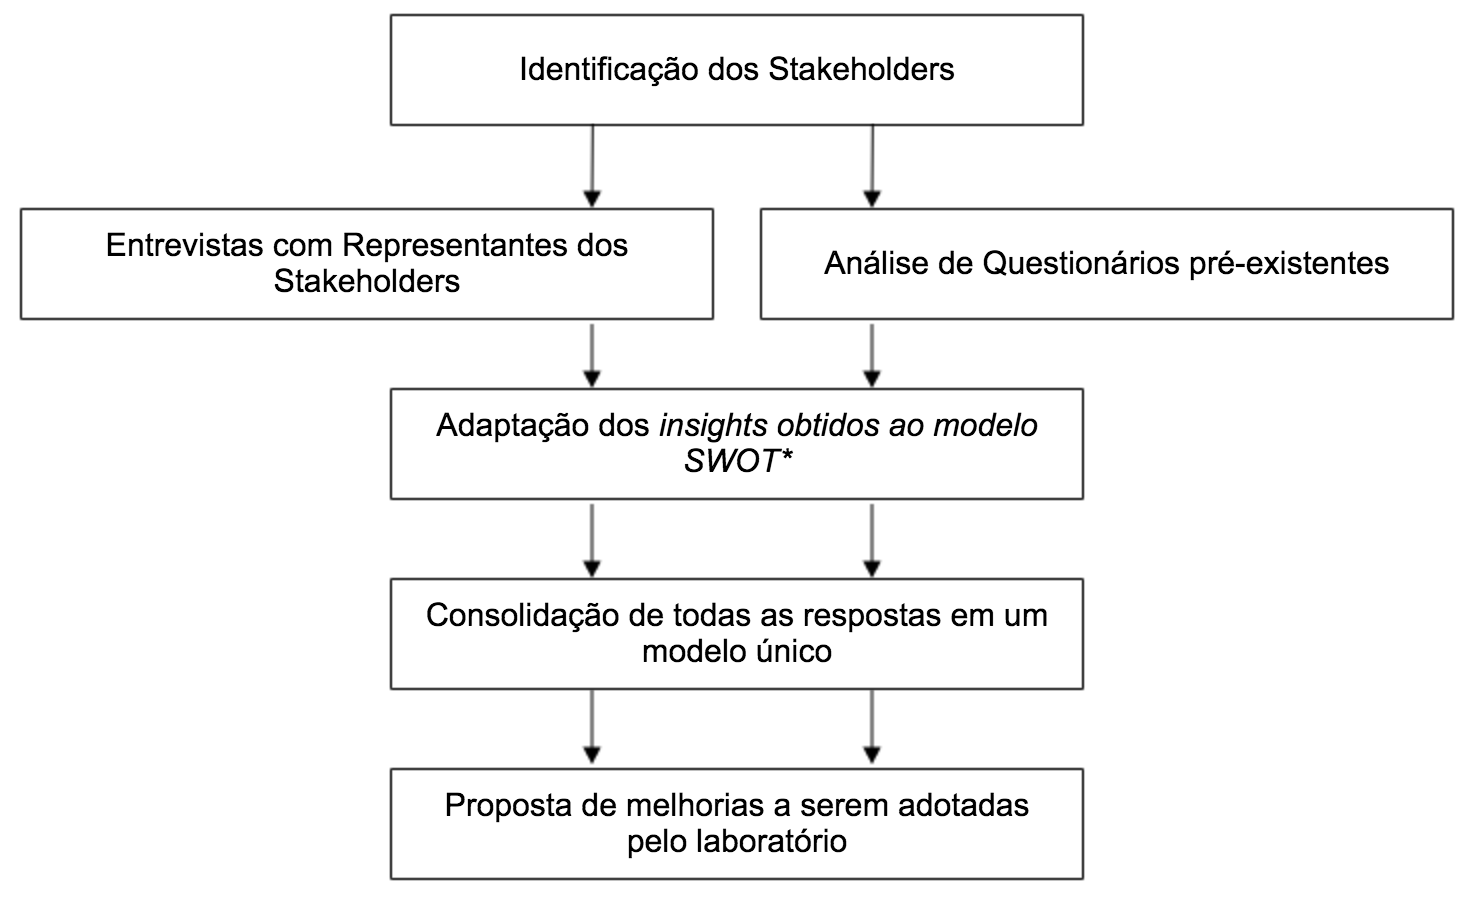
\includegraphics[scale=0.5]{img/metodologia}}
\label{fig:metodologia}
\caption* {Fonte: Elaborado pelo próprio autor}
\end{figure}

Após conversas iniciais com membros da Samsung e do PRO, foram definidos os stakeholders do projeto Ocean, juntamente com as pessoas-chave de cada. Foram realizadas entrevistas semi-estruturadas e gravadas, de forma a deixar a liberdade para serem feitas perguntas não presentes na estrutura inicial, e assim ter uma conversa guiada com o entrevistado como se não fosse uma entrevista formal. Antes de cada entrevista eram preparadas perguntas relacionadas ao mapeamento e percepção das interações do \textit{stakeholder} com o Ocean segundo a visão do entrevistador, e para todos os entrevistados era perguntado "se a pessoa teria alguma sugestão para a melhoria do Laboratório".

Em específico para os cursistas dos cursos básicos, o método de entrevistas foi considerado menos eficiente pelo alto número de interações com os participantes através das aulas. Portanto, foram aproveitados os questionários respondidos nos últimos dois anos de cursos - totalizando um total de 5280 respostas - para extrair as informações necessárias para este trabalho. O modelo de questionário aplicado encontra-se em anexo. No caso, foram analisadas somente as respostas das questões analíticas: "O que mais o motivou nesse curso?", "O que você acha que pode ser melhorado?" e "Qual tema você gostaria que fosse abordado num próximo curso?".

De forma a analisar e extrair informações desses questionários, o autor optou por desenvolver um software próprio para manipular esses dados via palavras-chave, pelos motivos elencados a seguir.

\begin{description}
\item [Volume de Dados] A quantidade de dados é grande o suficiente para dificultar - porém não inviabilizar - a leitura individual de cada uma das respostas. Acredita-se que mesmo que se optasse pela leitura individual, ela deveria ser acompanhada de uma \textit{clusterização} das respostas em categorias, o que a análise via repetição de palavras-chave também permite encontrar. Em contrapartida, os dados são suficientemente pequenos a ponto de não ser viável buscar alternativas  de \textit{Machine Learning} existentes para tratar esses dados, pois o volume não seria suficiente para treinar a inteligência artificial utilizada.

\item [Proposta do Estudo] Embora exista um campo muito grande de possibilidades de tratar e manipular os dados presentes, existe a necessidade de seguir com os objetivos inicias do presente estudo, que diz respeito ao posicionamento do Ocean de forma holística, e não somente na questão do aprendizado transmitido através de seus cursos. O autor acredita que há espaço para análises mais sofisticadas - dignas de um trabalho dedicado somente a isso - que poderiam ser realizadas caso a Samsung encontre a necessidade de entender os cursistas nos mínimos detalhes.

\item [Manipulação de Dados] O uso de uma ferramenta própria dá ao autor a liberdade de trabalhar e iterar em cima dos dados de forma a otimizar a ferramenta para o próprio uso. Existem disponíveis ferramentas prontas de geração de nuvens de palavras, que possuem um intuito muito maior de apresentar um 'choque visual' do que apresentar dados analíticos em si. A manipulação de dados permite que o autor encontre associações entre palavras ao observar os dados gerados pela ferramenta e trabalhar em cima da própria ferramenta para eliminar redundâncias ou dados inconsistentes.

\item [Princípio do Desenvolvedor] O princípio do desenvolvedor diz que se não há uma ferramenta própria que sirva para sua necessidade, desenvolva uma ferramenta que sirva. No caso, além de satisfazer com maior necessidade do que outras ferramentas presentes, é de satisfação do autor como desenvolvedor utilizar da programação para resolver problemas reais.
 
\end{description}

Vale destacar que os insights obtidos a partir desses modelos analíticos também são de grande valia para a Samsung, pois a parte qualitativa dos questionários nunca havia sido explorada anteriormente. 

Já para usuários de cursos intensivos, foram feitas entrevistas com representantes de \textit{startups} que frequentaram o curso anteriormente, centradas na pergunta: "Como a participação no curso intensivo mudou a vida da empresa e as vidas dos participantes?".

Para consolidar a análise realizada para cada \textit{stakeholder}, foi utilizada uma adaptação do modelo SWOT para ilustrar as percepções obtidas de cada um. Ela difere do modelo original do SWOT por não se tratar de uma análise de negócio baseada em fatores de mercado e competitividade, e sim em uma análise fria e absoluta de fatores básicos em um projeto: Pontos Fortes (\textit{Strengths}), Pontos Fracos (\textit{Weaknesses}), Oportunidades (\textit{Opportunities}) e Ameaças (\textit{Threats}). Foi considerado que por ser um modelo simples e de fácil visualização, consolidaria as necessidades deste trabalho sem desvirtuar os objetivos propostos.

\begin{figure}[h]
\caption{Quadro SWOT básico}
\centerline{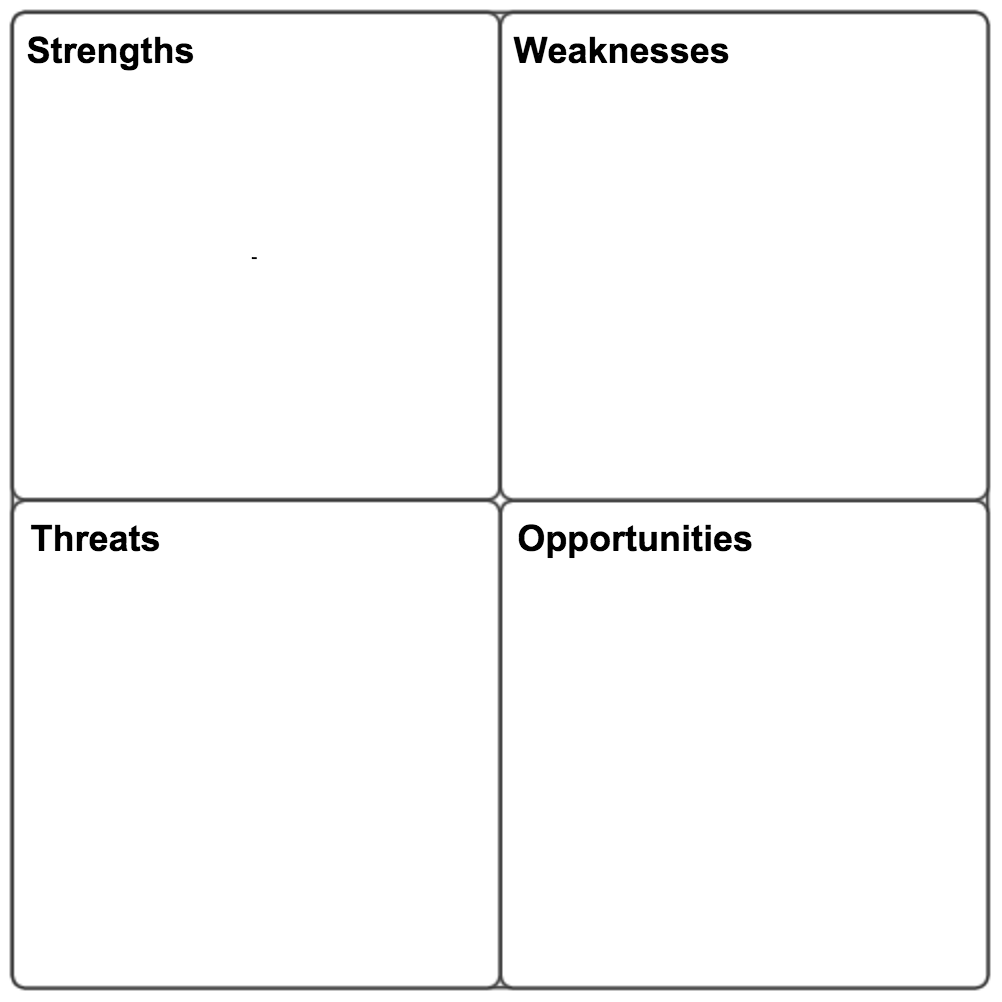
\includegraphics[scale=0.5]{img/detailedswot}}
\label{fig:detailedswot}
\caption* {Fonte: Quadro SWOT básico}
\end{figure}

A partir dos resultados obtidos pela análise das respostas, trabalhou-se em cima da geração de propostas de melhoria.